\section{The \fermi Gamma-ray Space Telescope}
\seclabel{fermi_telescope}

\begin{figure}[htbp]
  \centering
    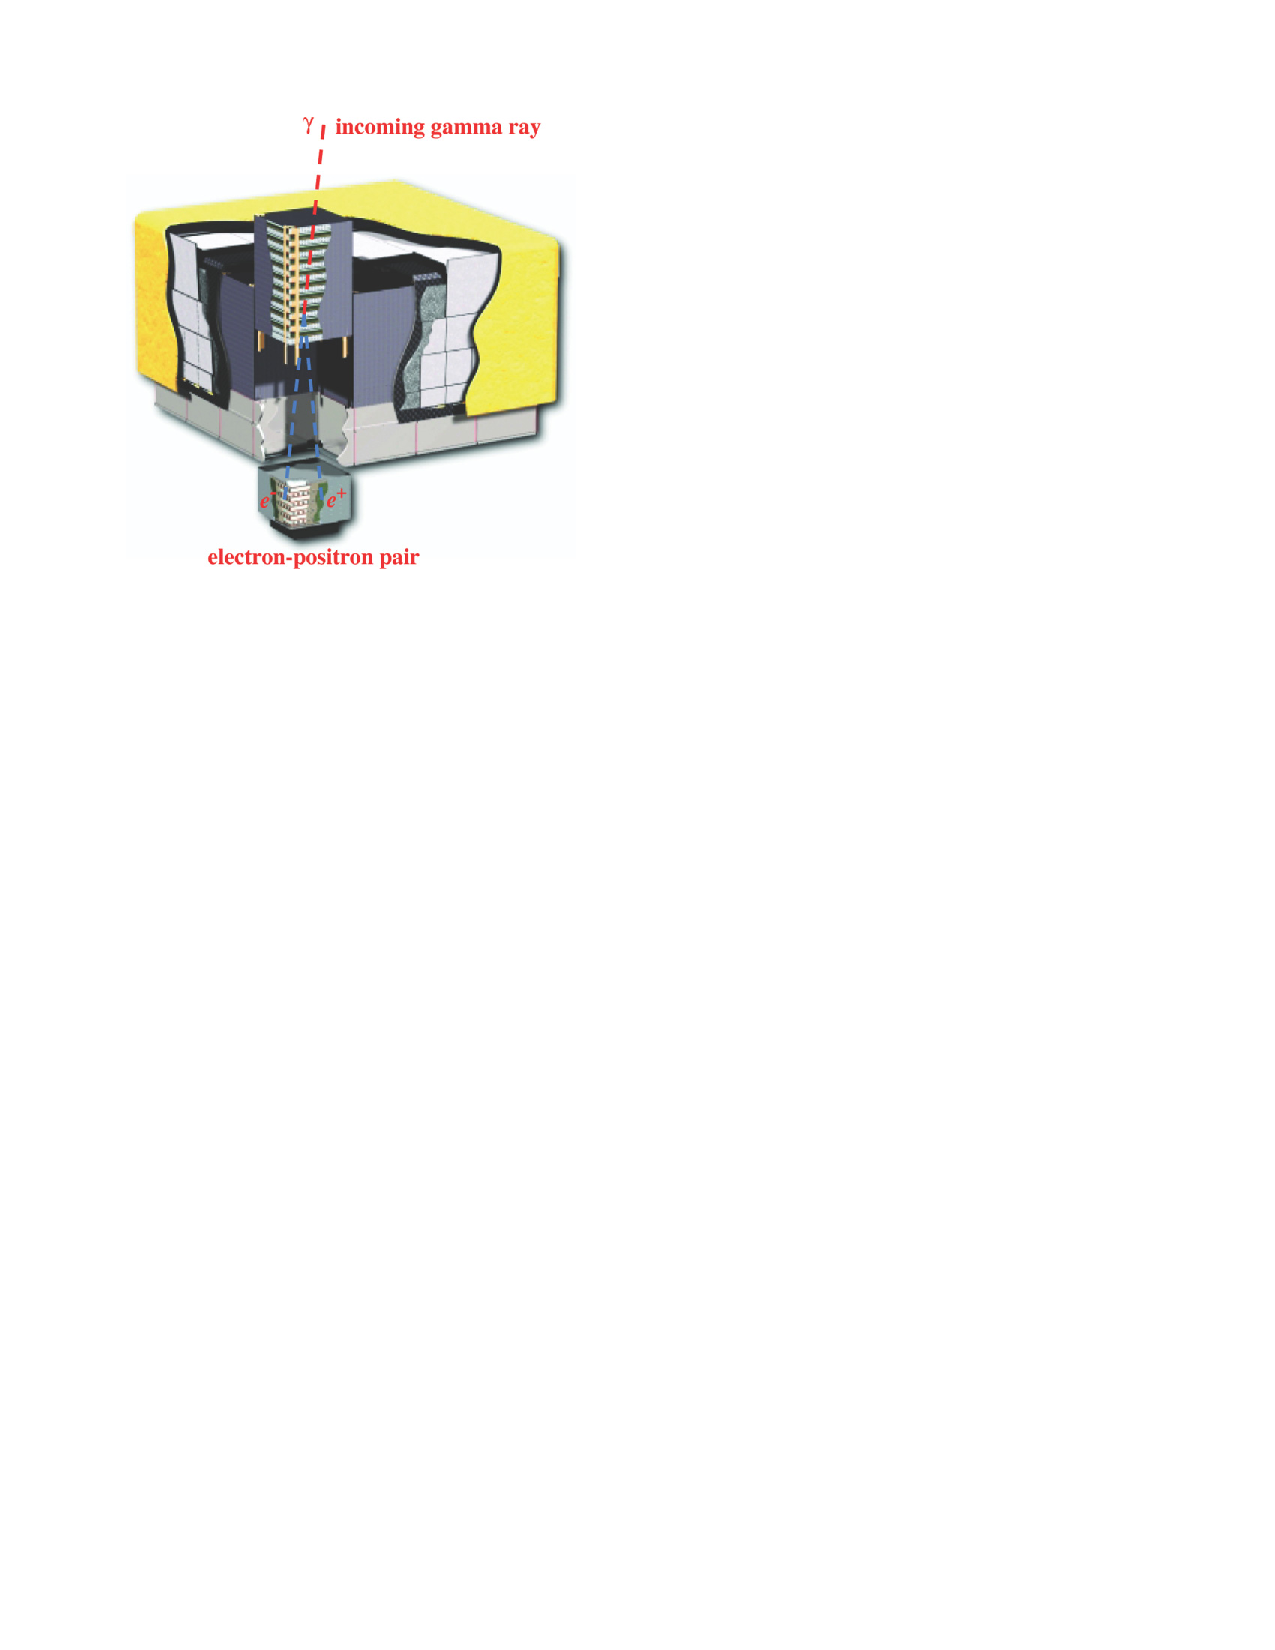
\includegraphics{chapters/introduction/figures/lat_detector_cutout.pdf}
  \caption{A schematic diagram of the \ac{LAT} with an incident $\gamma$-ray
    (red line) pair-converting into an electron and positron (blue lines)
    which are recorded in the tracker and calorimiter of the \ac{LAT}.
    This figure is taken from \citep{atwood_2009a_large-telescope}.  
    This diagram shows the three major subsystems of the \ac{LAT}:
    the tracker, the calorimiter, and the \ac{ACD}.
  }
  \figlabel{lat_detector_cutout}
\end{figure} 


The \fermi Gamma-ray Space telescope was launched on June 11, 2008 on
a Delta II heavy launch vehicle \citep{atwood_2009a_large-telescope}.
The primary since instrument on board \fermi is the \ac{LAT},
which is a pair-conversion telescope which detects $\gamma$-rays
in the energy range from $20\unitspace\mev$ to $>300\unitspace\gev$.
\figref{lat_detector_cutout} shows a schematic diagram of the \ac{LAT}.
With its unprecedent effective area and angular resolution, the \ac{LAT}
has drastically improved our understanding of the $\gamma$-ray sky.
In addition, \fermi contains the \Ac{GBM}, which is used to obseerve
\acp{GRB} in the energy range from $\sim8\unitspace\kev$ to $\sim40\unitspace\mev$.
See \cite{meegan_2009a_fermi-gamma-ray} for a description of the \ac{GBM}
detector.

\subsection{The \acs{LAT} Detector}

The \ac{LAT} is composed of three major subsystems: the tracker, the
calorimeter, and the \ac{ACD}. Fundamentally, the detector operates by
inducing an incident $\gamma$-ray to pair convert in the tracker into
an electron and positron pair. The electron and position travel through
the tracker and into the \ac{CsI} calorimiter.  The track they leave in
the tracker and the energy deposite they leave in the calorimter can be
used to infer the direction and energy of the incident $\gamma$-ray.

Both the tracker and calorimiter are $4\times4$ arrays, each composed of
16 modules.  Each tracker tower is divided into 18 tungsten converter
layers and 16 dual-silicon tracker planes ($x$ and $y$).  As a balance
between effective area and angular resolution, The top 12 tracker planes
have thin layers of tungsten which minimize the probability of secondary
scattering and improves the angular resolution of the \ac{LAT}, especially
for low-energy $\gamma$-rays. The bottom four tracker planes have layers
of tungsten $\sim6$ times thicker, which improves the likelihood of
conversion and therefore the effective area.  The ``front'' and ``back''
classificaiton for $\gamma$-rays refers to if they convert in the thin
or thick layers of the detector, respectivly.  Each calorimiter module
composed of eight layers of 12 \ac{CsI} crystals. The depth of the
calorimiter is 8.6 radiation lenghts adn the depth of entire insutrment
is 10.1 radiation lenths.

The \ac{ACD}, the third subsystem on the \ac{LAT}, provides provides
background rejection by of the charged particle background incident
on the \ac{LAT}.  The \ac{ACD} surrounds the tracker and is composed
of 89 plastic scintillator tiles ($5\times5$ on the top and 16
on each of the sides). The \ac{ACD} has a 0.9997 efficiency for
detcting singly-charged particles entering the \ac{LAT}.  A detailed
discussion of the various subsystems of the LAT can be found in
\citep{atwood_2009a_large-telescope}.

\subsection{Performance of the \acs{LAT}}
\subseclabel{performance_lat}

The \ac{LAT} 
has an unprecidended effective area ($\sim9,500\unitspace\cm^2$),
single-photon energy resolution ($\sim10\%$), and single-photon
angular resolution ($\sim3\fdg5$ at $\energy=100\unitspace\mev$
and decreasing to $\lesssim0\fdg15$ for $\energy>10\unitspace\gev$)
\citep{atwood_2009a_large-telescope}.

\begin{figure}[htbp]
  \centering
  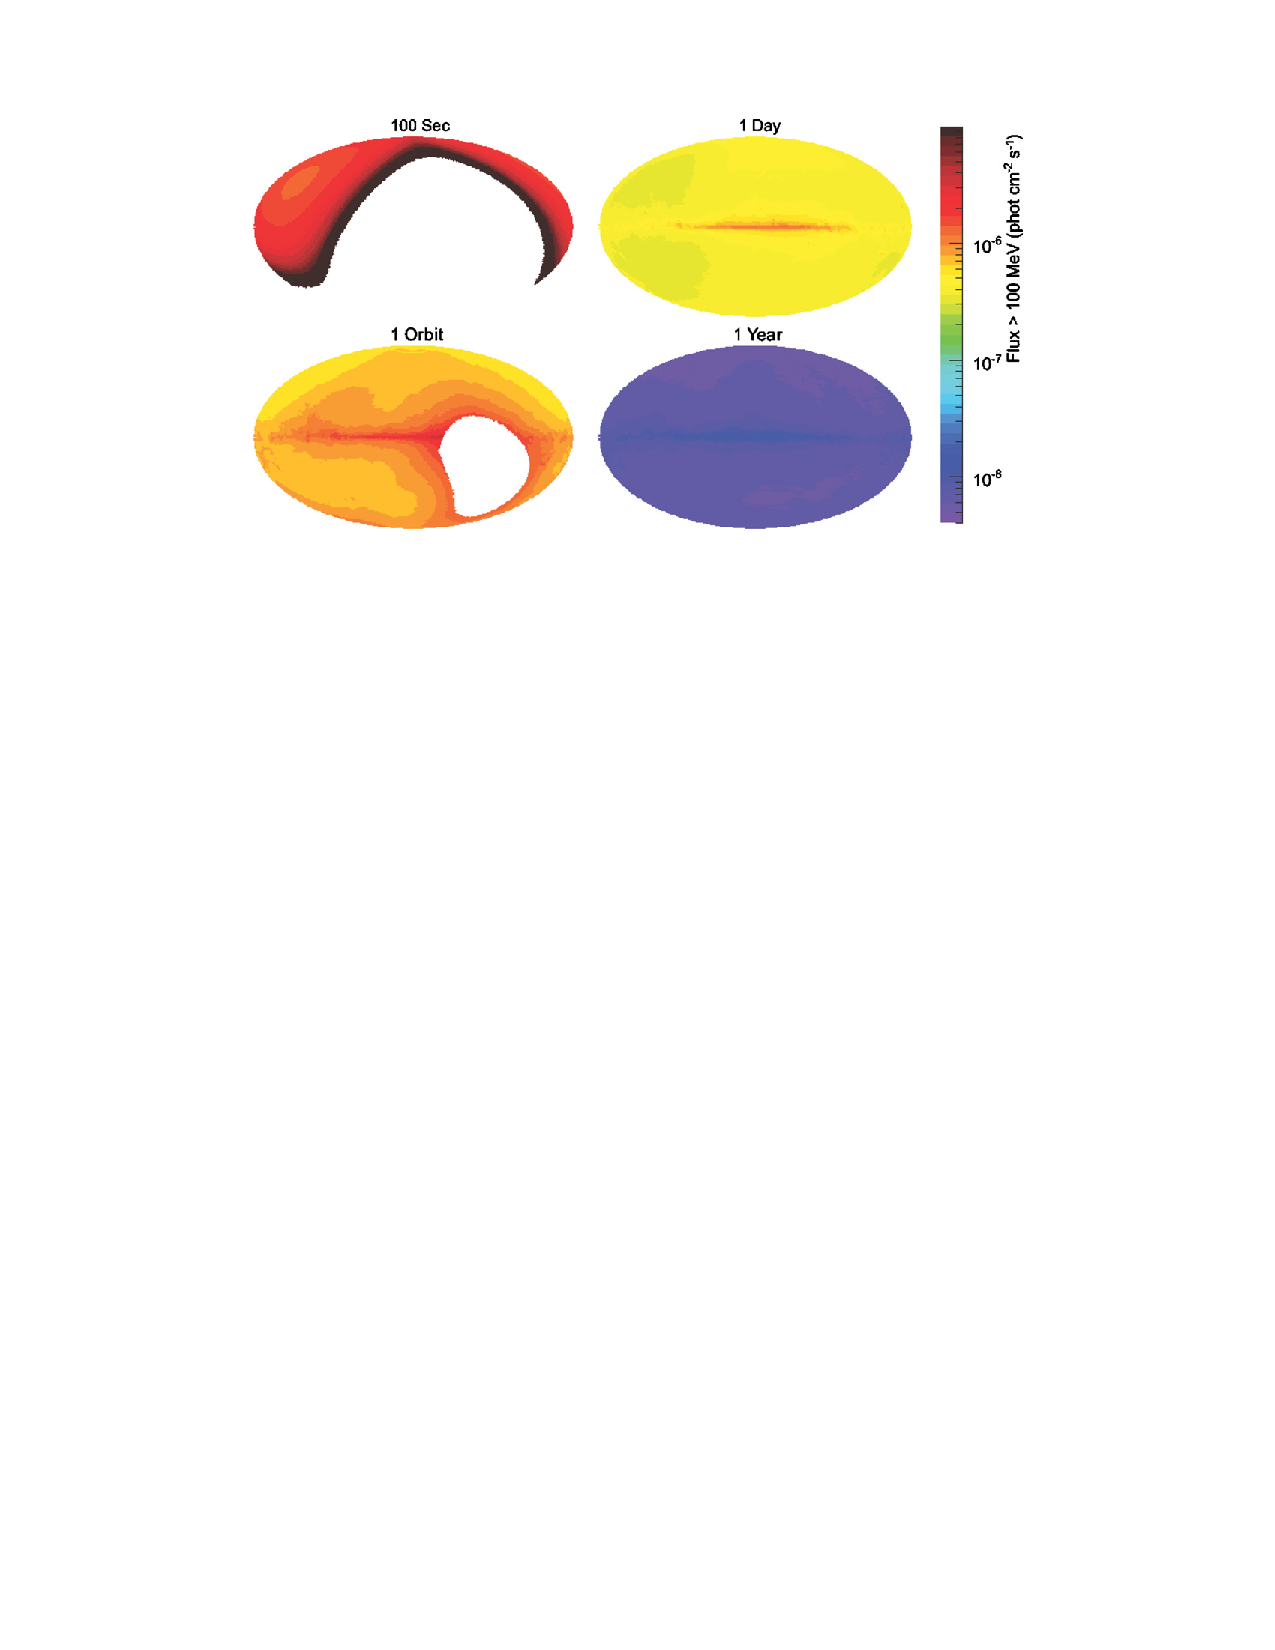
\includegraphics{chapters/introduction/figures/lat_point_source_sensitivity.pdf}
  \caption{
  The \ac{LAT} point-source sensitivity for exposures of
  $100\unitspace\second$, 1 orbit, $1\unitspace\dayunit$,
  and $1\unitspace\yearunit$.  This figure is from
  \cite{atwood_2009a_large-telescope}.
  }
  \figlabel{lat_point_source_sensitivity}
\end{figure} 


With its $2.4\unitspace\steradian$ filed of view, \fermi can observe
the entire sky almost unifomly every $\sim3\unitspace\hour$.
With one year of observations, the \ac{LAT} has a point-source
flux sensitivity ($E>100\unitspace\mev$) of $3 \times 10^{-9}
\ph \cm^{-2}\second{-1}$ assuming a high-latitidue diffuse flux
($E>100\unitspace\mev$) of $1.5\times10^{-5}\cm^{-2}\second^{-1}\steradian^{-1}$
\figref{lat_point_source_sensitivity} plots the sensitivity
for exposures of varying timescales.


\begin{figure}[htbp]
  \centering
  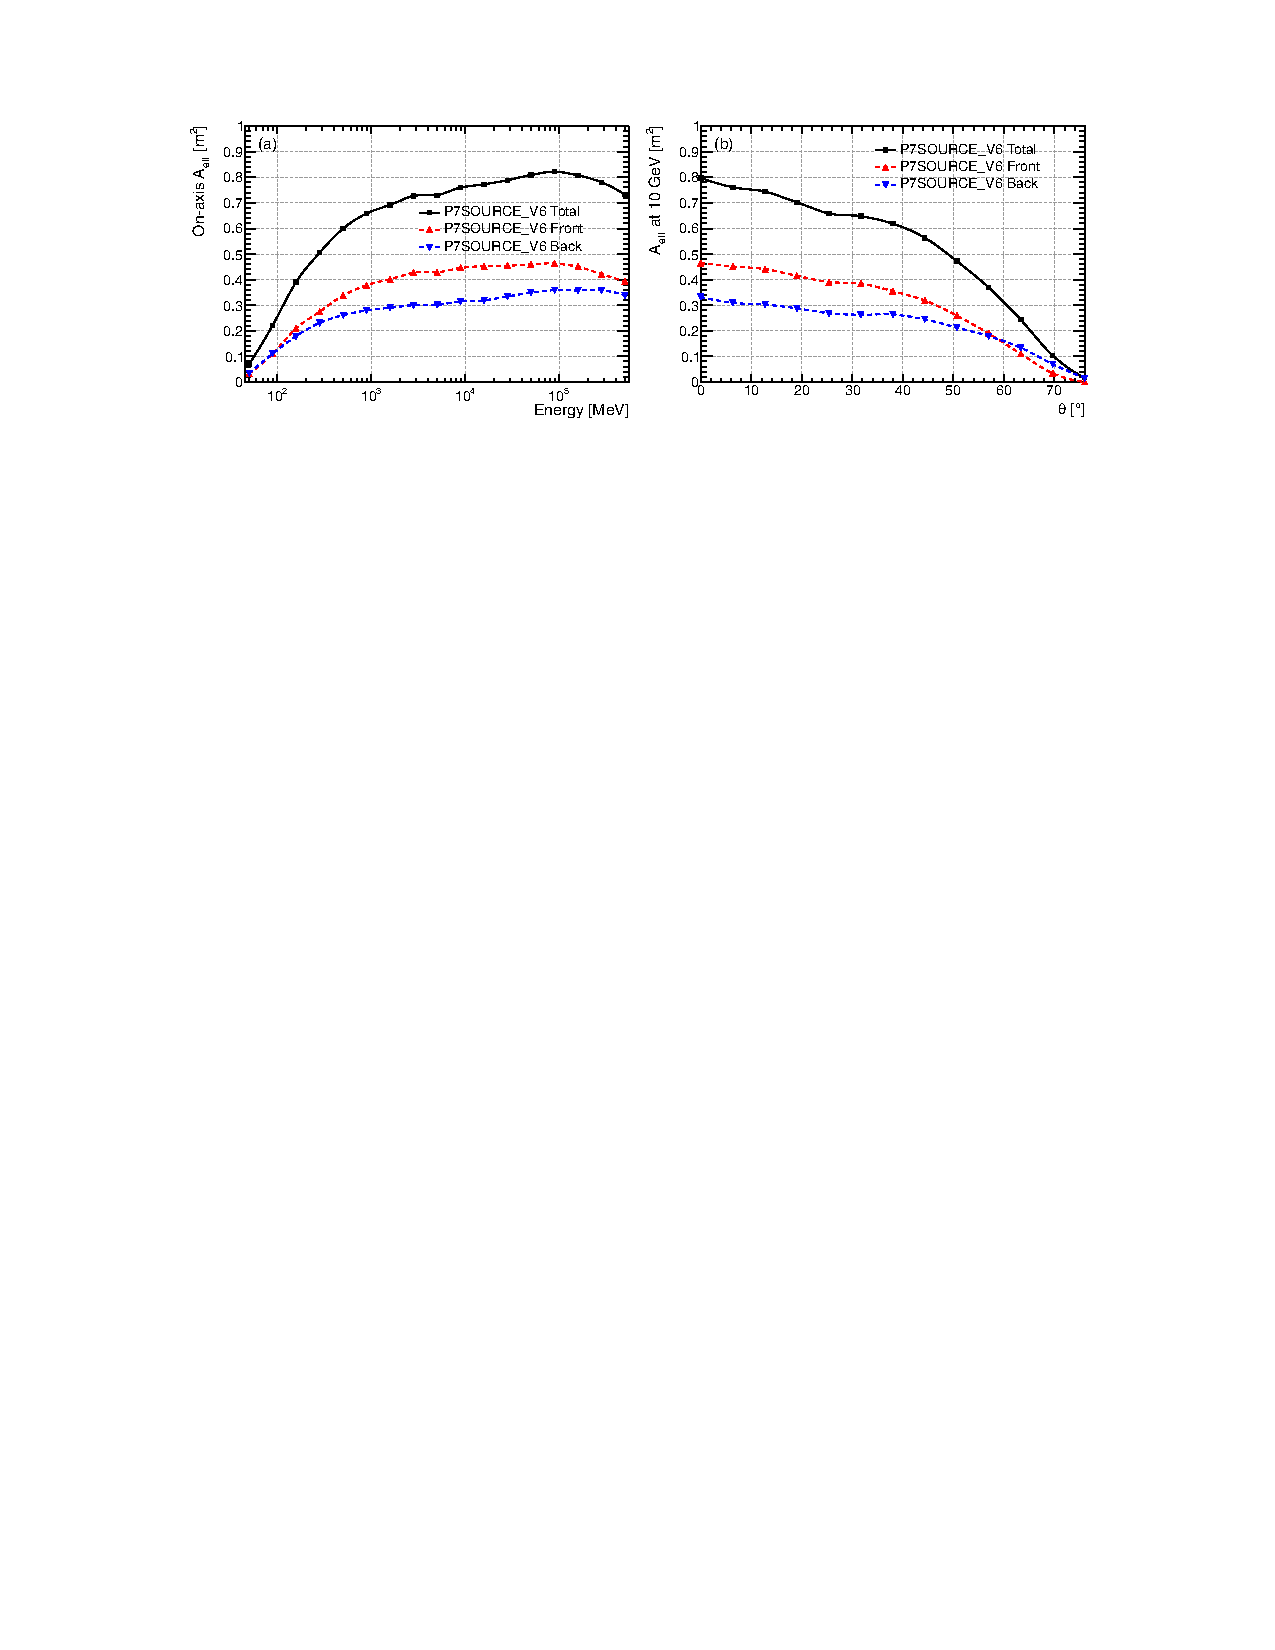
\includegraphics{chapters/introduction/figures/lat_effective_area.pdf}
  \caption{
  The \ac{LAT} effecitve area (a) as a function of energy for
  $\gamma$-rays that are incident on the \ac{LAT} perpendicularly from
  above and (b) as a function of incident angle for photons with an
  energy of $10\unitspace\gev$.  The \ac{LAT} performance is computed
  for the \psevensourcevsix event classification.  This figure is from
  \cite{ackermann_2012a_fermi-large}.
  }
  \figlabel{lat_effective_area}
\end{figure} 

\begin{figure}[htbp]
  \centering
  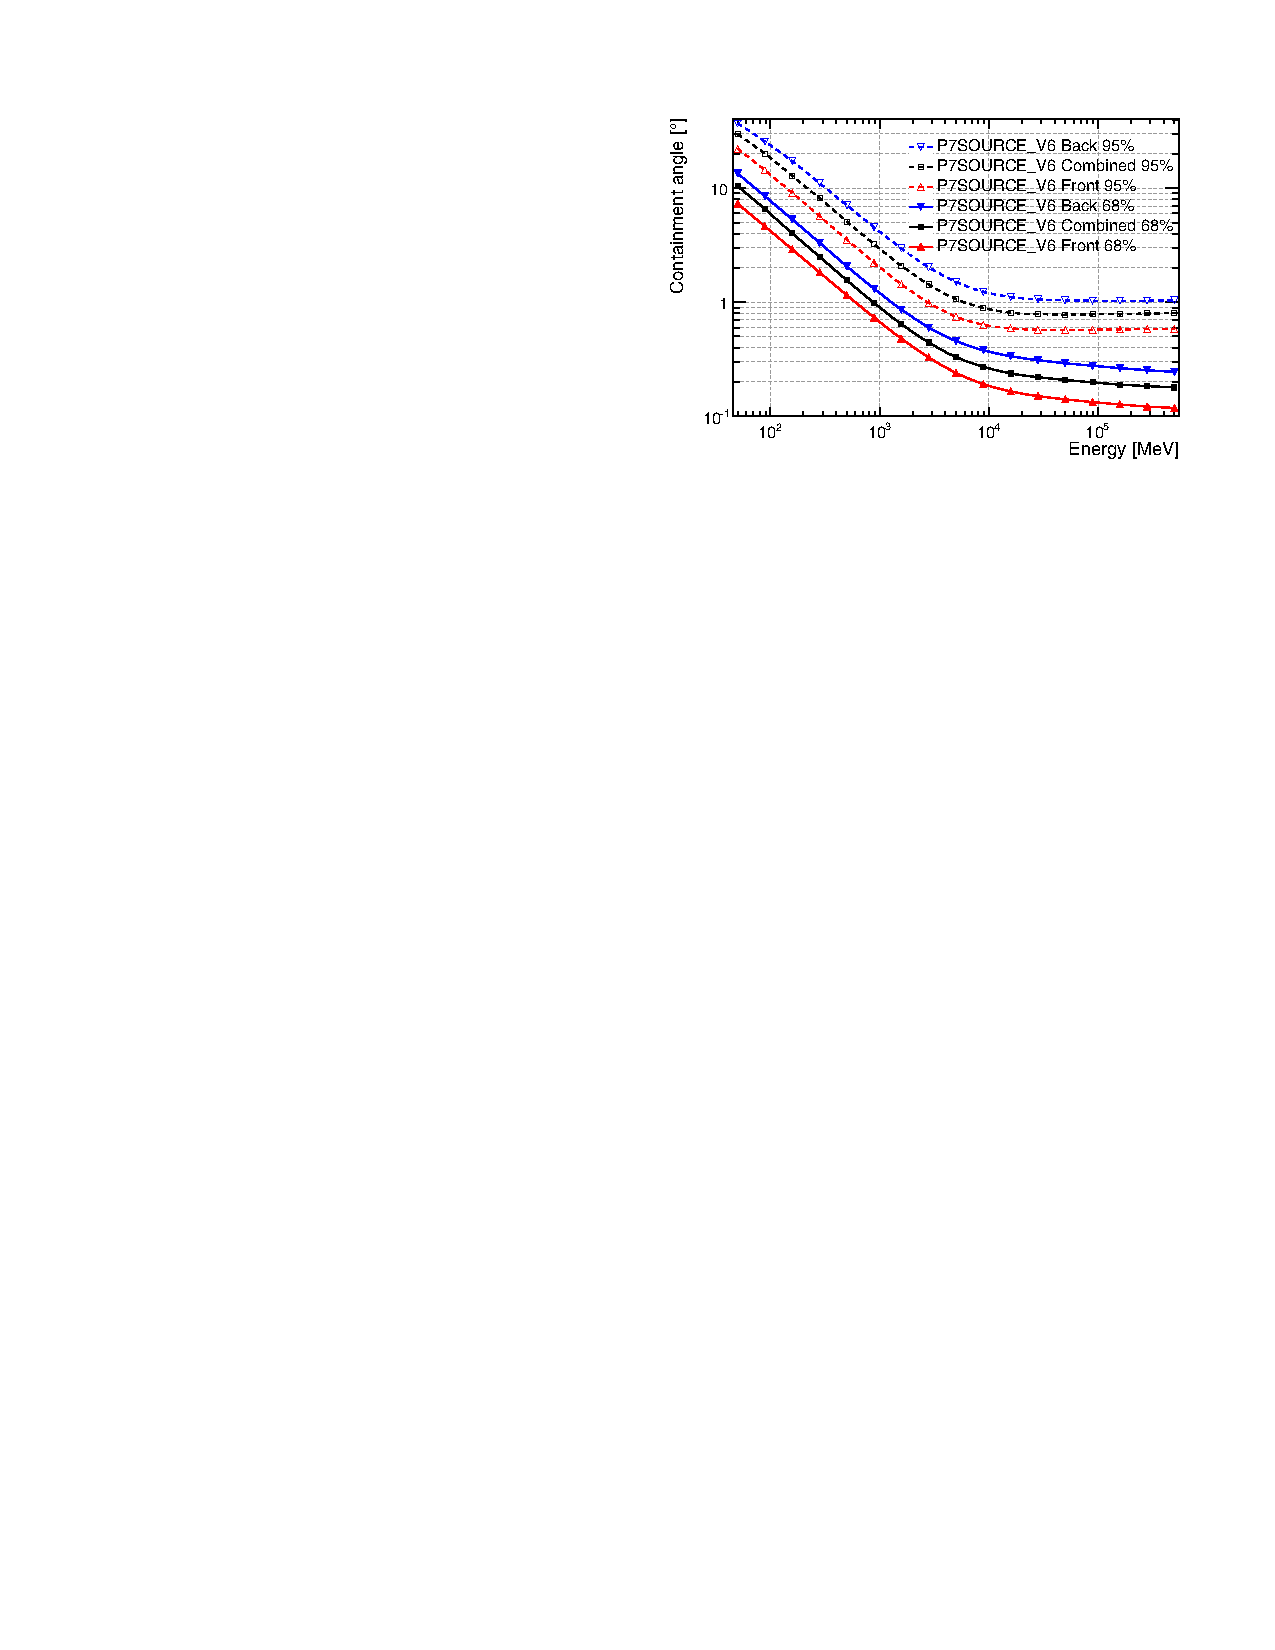
\includegraphics{chapters/introduction/figures/lat_psf.pdf}
  \caption{
  The angular resolution (68\% and 95\% containment radius)
  as a function of energy.
  The \ac{LAT} performance is computed for the \psevensourcevsix
  event classification.
  This figure is from \cite{ackermann_2012a_fermi-large}.
  }
  \figlabel{lat_psf}
\end{figure} 


\begin{figure}[htbp]
  \centering
  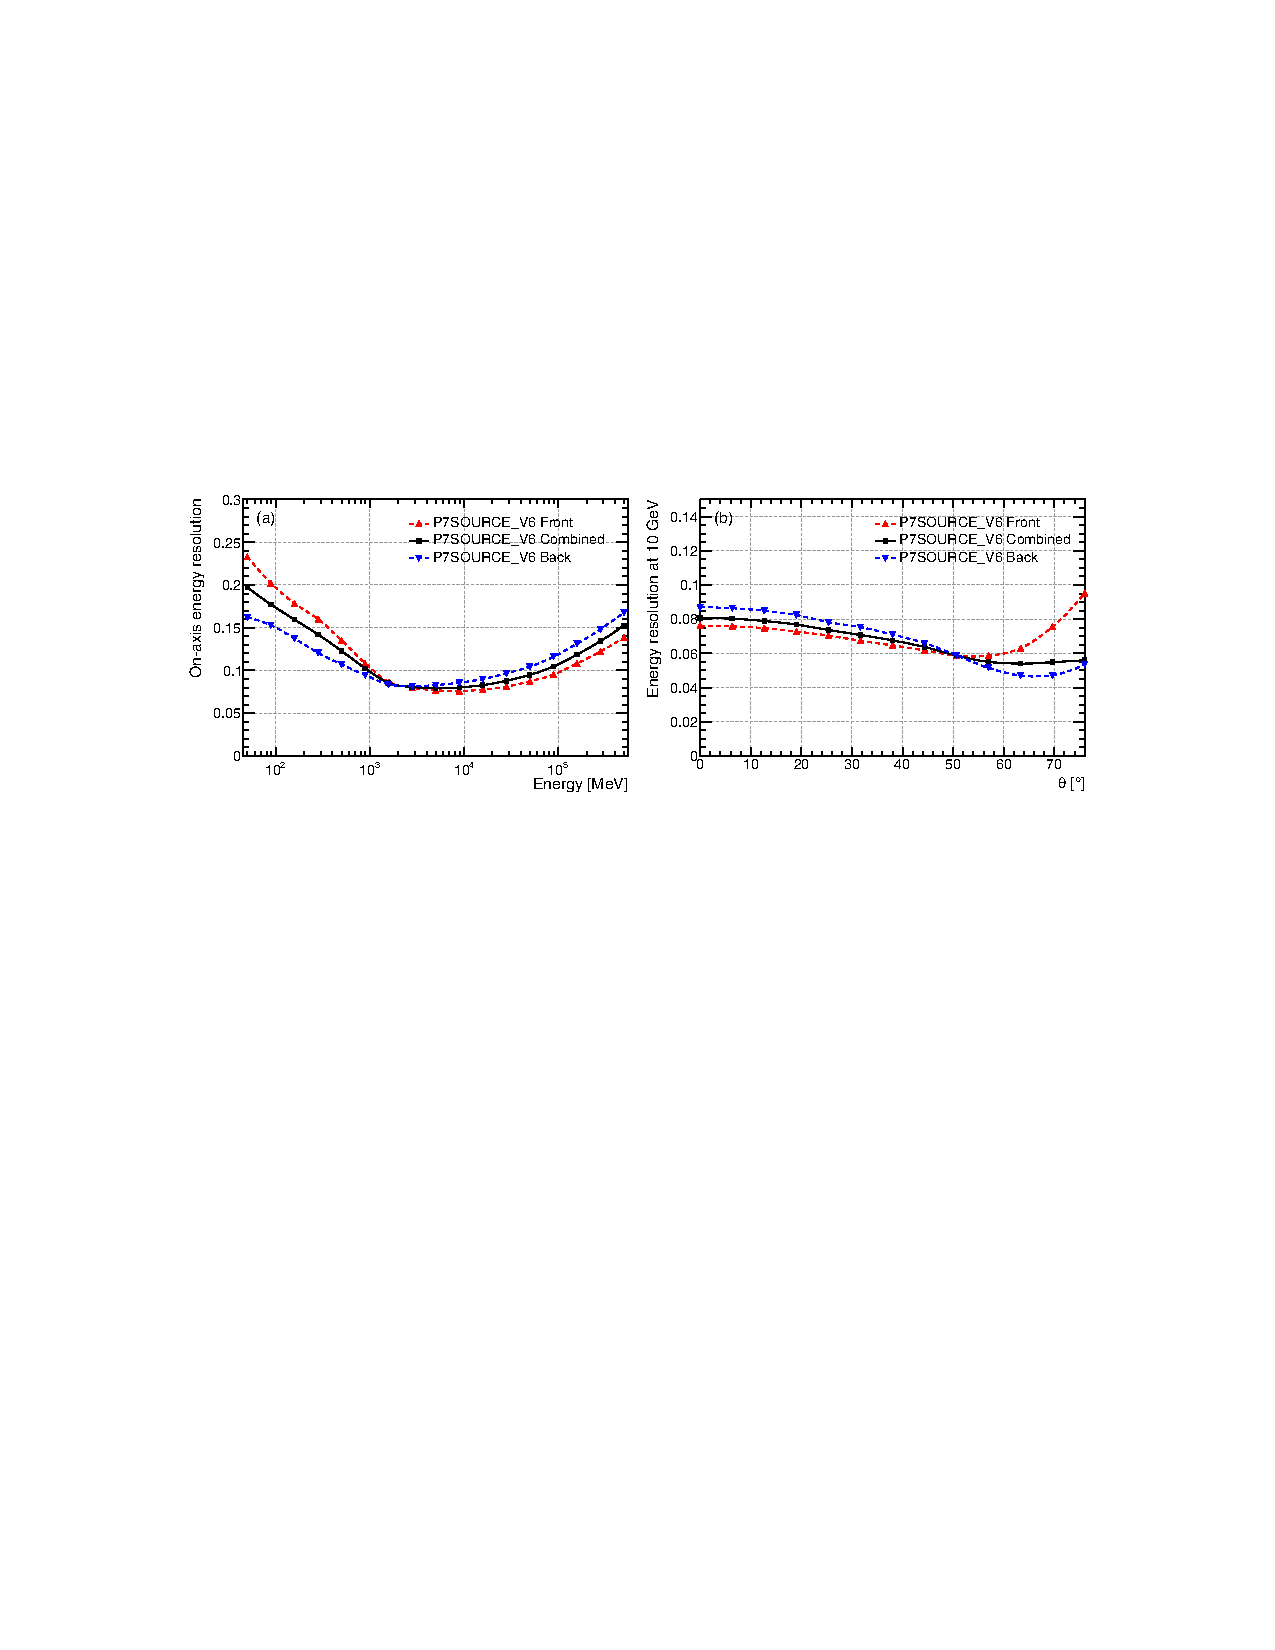
\includegraphics{chapters/introduction/figures/lat_energy_dispersion.pdf}
  \caption{
  The energy disperion (a) as a function of energy for $\gamma$-rays that
  are incident on the \ac{LAT} perpendicularly from above and (b) as a function
  of the incident angle for photons with an energy of $10\unitspace\gev$.
  The \ac{LAT} performance is computed for the \psevensourcevsix
  event classification.
  This figure is from \cite{ackermann_2012a_fermi-large}.
  }
  \figlabel{lat_energy_dispersion}
\end{figure} 

The effective area, \ac{PSF}, and energy dixpersion are both a function
of energy and of incident angle.  \figref{lat_effective_area}
plots the effective area as a function of energy and incident angle.
\figref{lat_psf} plots the \ac{PSF} as a function of energy.  Finally,
\figref{lat_energy_dispersion} plots the energy disperison as a function
of energy and incident angle.  Given the strongly-nonlinear response of
the \ac{LAT}, we will describe in \chapref{maximum_likelihood_analysis}
the analysis methods used to analyze \ac{LAT} data.


